\documentclass{article}
\usepackage[utf8]{inputenc}
\usepackage{graphicx}

\title{Operating Systems Notes}
\author{Jacob Burley} %add your name here if you're a collaborator
\date{12 December 2017}

\begin{document}

\graphicspath{ {/} }

\maketitle
\section{Introduction}
Operating System runs in kernel mode (supervisor mode), User programs run in User Mode
\\Instructions that control the machine or us I/O aren't available to User Mode (at least not directly)
\\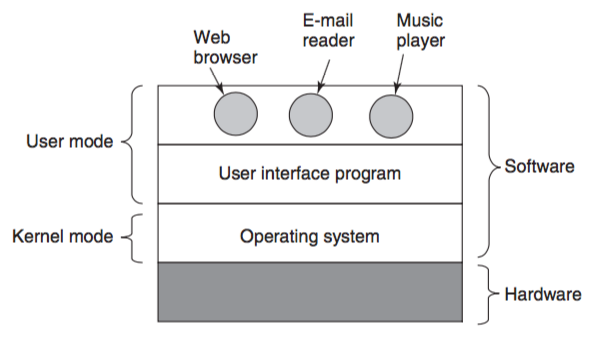
\includegraphics[width= 250pt]{ch1/1-1.png}
\\Operating System runs on bare hardware
\\OS extends hardware of a computer, and makes it easier for programmers to develop applications without having to deal with things like SATA interfaces directly
\\OS also provides abstractions for devices, files etc.
\\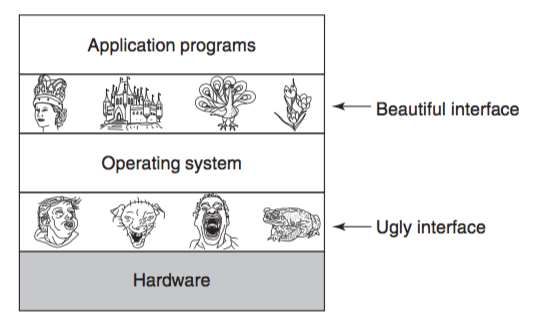
\includegraphics[width = 250pt]{ch1/1-2.png}
\\OS also manages hardware resources like CPU and RAM, as well as I/O
\section{Processes & Threads}

\section{Memory Management}

\section{File Systems}

\section{I/O}

\section{Deadlocks}

\end{document}